\pgfplotsset{width=12cm,compat=1.9}

\pgfplotsset{
  log ticks with fixed point,
}

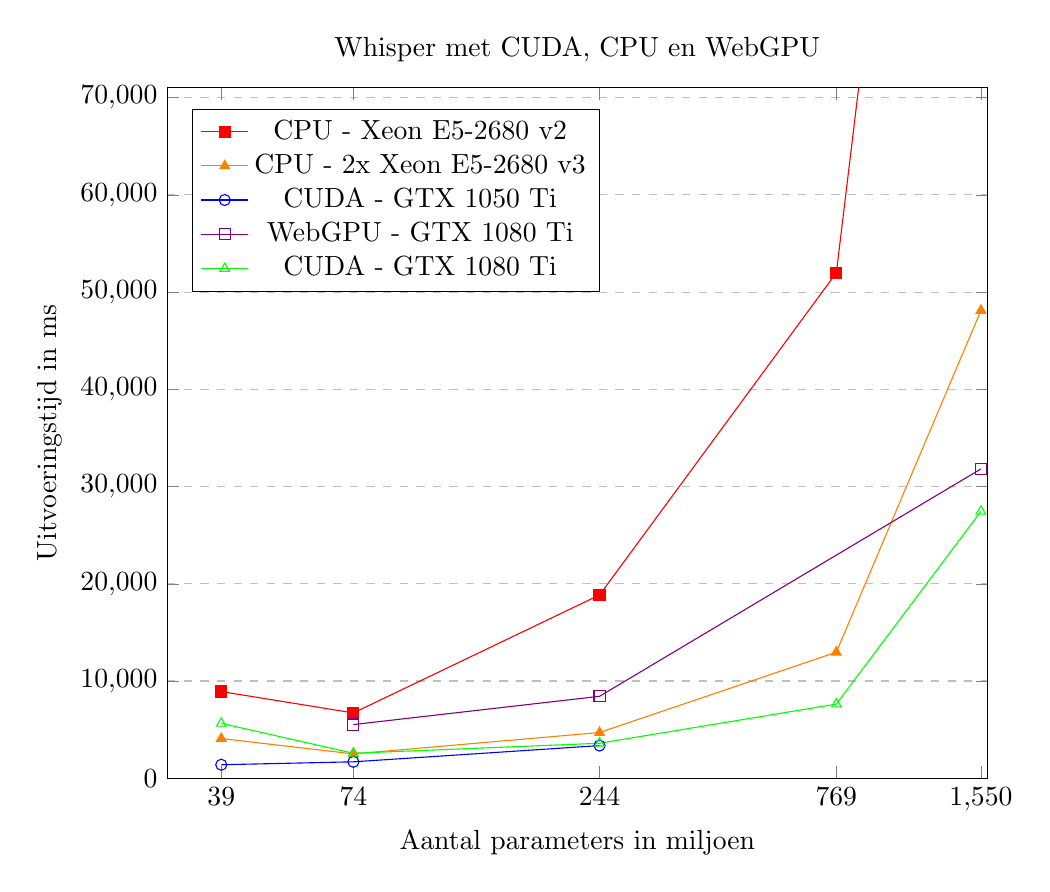
\begin{tikzpicture}
    \begin{semilogxaxis}[
        title={Whisper met CUDA, CPU en WebGPU},
        xlabel={Aantal parameters in miljoen},
        ylabel={Uitvoeringstijd in ms},
        xmin=30, xmax=1600,
        ymin=0, ymax=71000,
        xtick={39, 74, 244, 769, 1550},
        legend pos=north west,
        ymajorgrids=true,
        grid style=dashed,
        yticklabel style={
            /pgf/number format/fixed,
        },
        scaled y ticks=false
    ]
    \addplot[
            color=red,
            mark=square*
        ]
        coordinates {(39,8919)(74,6721)(244,18849)(769,51980)(1550,175378)};
        \addlegendentry{CPU - Xeon E5-2680 v2}
    \addplot[
        color=orange,
        mark=triangle*
        ]
        coordinates {(39,4088)(74,2508)(244,4706)(769,12963)(1550,48107)};
        \addlegendentry{CPU - 2x Xeon E5-2680 v3}
    \addplot[
            color=blue,
            mark=o
        ]
        coordinates {(39,1393)(74,1694)(244,3362)};
        \addlegendentry{CUDA - GTX 1050 Ti}
    \addplot[
            color=violet,
            mark=square
        ]
        coordinates {(74,5526)(244,8431)(1550,31814)};
        \addlegendentry{WebGPU - GTX 1080 Ti}
    \addplot[
            color=green,
            mark=triangle
        ]
        coordinates {(39,5647)(74,2574)(244,3602)(769,7629)(1550,27448)};
        \addlegendentry{CUDA - GTX 1080 Ti}
    \end{semilogxaxis}
\end{tikzpicture}